\section{Construcción del corpus}

\subsection{Extracción}
\begin{frame}
    \frametitle{Extracción}

    \begin{itemize}
        \item Humor: se busca en Twitter por la palabra clave \emph{chiste} y se eligen cuentas, llegando a 16.333 tweets.
        \item No humor: cuentas de noticias, frases filosóficas y curiosidades, alcanzando los 25.755 tweets.
    \end{itemize}
\end{frame}

\subsection{Anotación}
\begin{frame}[allowframebreaks]
    \frametitle{Anotación}

    \begin{itemize}
        \item Hay una excesiva cantidad de tweets para filtrar.
        \item Se crea una aplicación para que usuarios los anoten.
    \end{itemize}

    \framebreak

    \begin{center}
        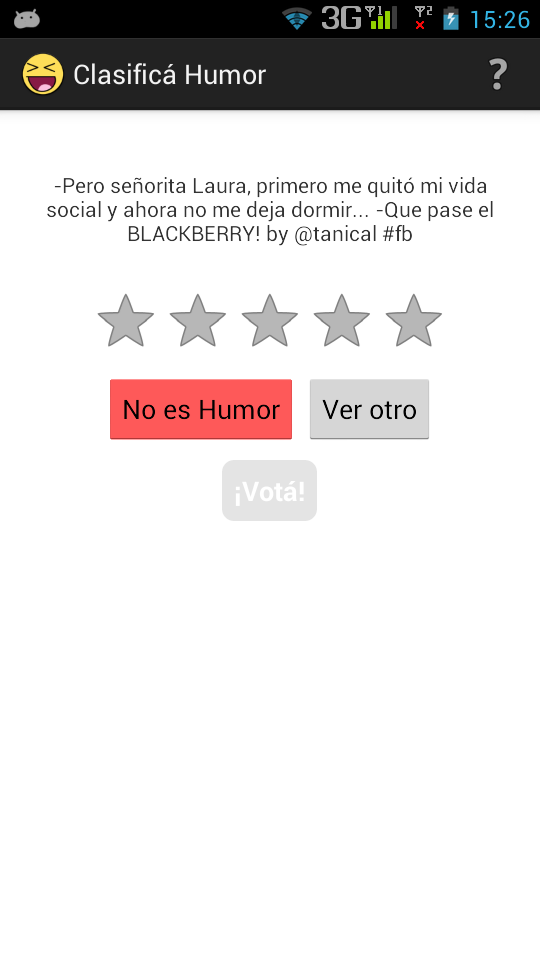
\includegraphics[frame, height=6cm]{app.png}
        \hspace{1cm}
        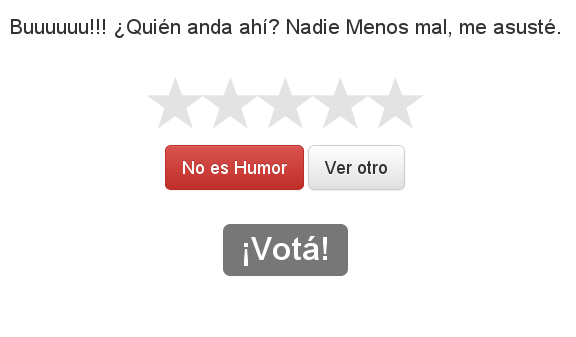
\includegraphics[frame, height=6cm]{pagina.png}
    \end{center}

    \framebreak

    \begin{itemize}
        \item Cantidad de clases a considerar
        \item Contenido
        \item Eficiencia
        \item Algoritmo de selección
    \end{itemize}
\end{frame}
